\begin{figure}[htbp]
\centering
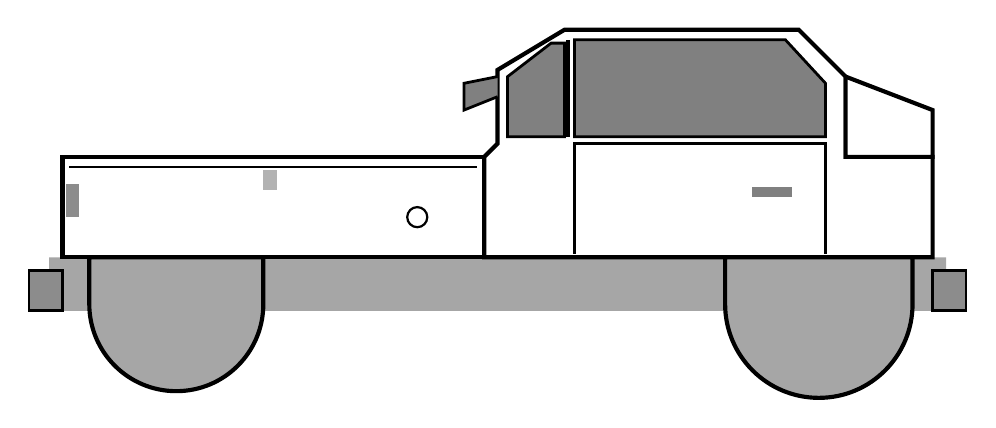
\begin{tikzpicture}[scale=0.85]

    % === WHEELS ===
    % Rear wheel
    \draw[line width=1.5pt, black, fill=black!70] (2.2,1.1) circle (1.1);
    \draw[line width=1pt, black, fill=black!45] (2.2,1.1) circle (0.65);

    % Front wheel
    \draw[line width=1.5pt, black, fill=black!70] (11.8,1.1) circle (1.1);
    \draw[line width=1pt, black, fill=black!45] (11.8,1.1) circle (0.65);

    % === LOWER BODY / ROCKER PANEL (gray area) ===
    \fill[black!35]
        (0.3,1.0) -- (0.3,1.8) -- (1.0,1.8) --
        (1.0,1.1) arc (180:360:1.2) -- (3.4,1.1) -- (3.4,1.8) --
        (10.5,1.8) -- (10.5,1.1) arc (180:360:1.3) -- (13.1,1.1) --
        (13.1,1.8) -- (13.7,1.8) -- (13.7,1.0) -- cycle;

    % === MAIN BODY (white with black outline) ===

    % Truck bed
    \draw[line width=1.5pt, black, fill=white]
        (0.5,1.8) -- (0.5,3.3) -- (6.8,3.3) -- (6.8,1.8) -- cycle;

    % Bed inner line (top edge detail)
    \draw[line width=1pt, black] (0.6,3.15) -- (6.7,3.15);

    % Cab
    \draw[line width=1.5pt, black, fill=white]
        (6.8,1.8) -- (6.8,3.3) -- (7.0,3.5) -- (7.0,4.6) --
        (8.0,5.2) -- (11.5,5.2) -- (12.2,4.5) -- (12.2,3.3) --
        (13.5,3.3) -- (13.5,1.8) -- cycle;

    % Hood
    \draw[line width=1.5pt, black, fill=white]
        (12.2,3.3) -- (12.2,4.5) -- (13.5,4.0) -- (13.5,3.3) -- cycle;

    % === WINDOWS ===

    % Rear cab window
    \draw[line width=1pt, black, fill=black!50]
        (7.15,3.6) -- (7.15,4.5) -- (7.8,5.0) -- (8.0,5.0) -- (8.0,3.6) -- cycle;

    % Side window
    \draw[line width=1pt, black, fill=black!50]
        (8.15,3.6) -- (8.15,5.05) -- (11.3,5.05) -- (11.9,4.4) -- (11.9,3.6) -- cycle;

    % Window frame/pillar
    \draw[line width=1.5pt, black] (8.05,3.6) -- (8.05,5.05);

    % === DOOR ===
    \draw[line width=1pt, black] (8.15,1.85) -- (8.15,3.5) -- (11.9,3.5) -- (11.9,1.85);

    % Door handle
    \fill[black!50] (10.8,2.7) rectangle (11.4,2.85);

    % === WHEEL WELLS (gray arches) ===
    % Rear wheel well
    \draw[line width=1.5pt, black, fill=black!35]
        (0.9,1.8) -- (0.9,1.1) arc (180:360:1.3) -- (3.5,1.8) -- cycle;

    % Front wheel well
    \draw[line width=1.5pt, black, fill=black!35]
        (10.4,1.8) -- (10.4,1.1) arc (180:360:1.4) -- (13.2,1.8) -- cycle;

    % === BUMPERS ===
    % Rear bumper
    \fill[black!45] (0.0,1.0) rectangle (0.5,1.6);
    \draw[line width=1pt, black] (0.0,1.0) rectangle (0.5,1.6);

    % Front bumper
    \fill[black!45] (13.5,1.0) rectangle (14.0,1.6);
    \draw[line width=1pt, black] (13.5,1.0) rectangle (14.0,1.6);

    % === SIDE MIRROR ===
    \fill[black!50] (7.0,4.2) -- (6.5,4.0) -- (6.5,4.4) -- (7.0,4.5) -- cycle;
    \draw[line width=1pt, black] (7.0,4.2) -- (6.5,4.0) -- (6.5,4.4) -- (7.0,4.5);

    % === TAILLIGHT ===
    \fill[black!45] (0.55,2.4) rectangle (0.75,2.9);

    % === DETAILS ===
    % Gas cap area
    \draw[line width=0.8pt, black] (5.8,2.4) circle (0.15);

    % Bed stake hole
    \fill[black!30] (3.5,2.8) rectangle (3.7,3.1);

\end{tikzpicture}
\caption{Classic pickup truck profile used for quarter-car suspension analysis.}
\label{fig:pickup_truck_profile}
\end{figure}
